\section{Google's Kubernetes:}
\label{sec:kubernetes}
Google's Kubernetes is an open source container orchestration tool which is built on the experience of 15 years of running production workloads at large scale. As a container management framework, it deploys containerized application using Docker containers and provides application scaling, scheduling of containers, routing of traffic, load balancing and container monitoring. 

Kubernetes implements the master-slave architecture. In Kubernetes cluster, one node works as the Kubernetes Master node which is responsible for coordinating with other nodes called as worker nodes. Worker nodes are the nodes in the cluster which actually runs the requested applications using containers. Each of these worker nodes runs an agent process, called kubelet, which talks to master node.

Master node runs a scheduler service. The scheduler service is used to monitor the resources and the workload on the worker nodes. Based on the available resources, it schedules the applications in a container on a node in the cluster. 

Containerized applications are not deployed directly on the nodes. They are assigned to pods. Pods are the basic unit on a worker node which represents related containers grouped together. Pods are basically a group of containers which act as a single application.

\begin{figure*}
\centering
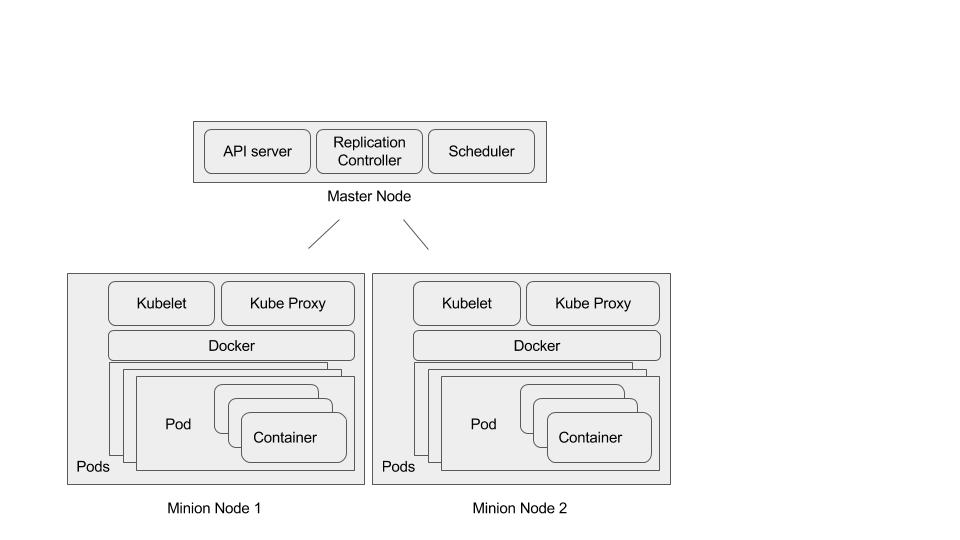
\includegraphics[scale=0.5]{./fig/kubernetes}
\caption{Google Kubertnetes Architecture}
\label{fig:kubernetesArch}
\end{figure*}

Following are the features of Kubernetes:

\begin{enumerate}
\item Pods:
A container is launched inside the smallest deployable unit called pods. One single pod can run multiple containers in it. These containers in one single pod share the network namepsace and pod's IP address. Each Pod has their own IP addresses. However, pod's network space is flat i.e. they don't need NAT to communicate with each other.

\item Service:
A group of pods having the same functionalities are called service. They run an application as a service which is used by other applications without knowing its lower details. The pods in a  service are associated and discovered using the labels (explained below). Load balancer, one of the services of Kubernetes, balances the workload among the associated pods. If one of the pods having too much workload, then load-balancing service will use kube-proxy to balance the workload. Kube-proxy will forward it to any of the less loaded pods in the same service. Kube-proxy are the network proxy that runs on every worker nodes.

\item Labels:
Pods can be labeled using a key/value data. This labels are user-defined tags on the pods. Labeling is not limited to the pods. A service running in Kubernetes can also be labeled. 

\item Replication Controller:
Pods can be replicated to provide availability using replication controller running on the master node. The replication controller replicates the pods using the pod template. It also maintains the pod's replicas using the labels tagged on the related pods. If one of them dies, replication controller will create another pod using the template. Replication controller can also scale down the pods. 

\item Volumes:
Since the containers are ephemeral, it is needed to recover the files residing on the failed container to restart it from its failed state. Kubernetes achieve this by supporting the concept of volumes. volume is an abstraction type which is basically a directory at the core level. The volume lives as long as the pod is alive and the data in the volume is maintained even if a container fails.

\item ETCD and state management:
Etcd is a service running on the master node which is used to store the configuration data in key/value pair distributed over the cluster. It is used state management and service discovery. 

\item API server:
Kubernetes provides users an API server running on master node to configure workloads and containers. API server is based on RESTful interface allowing different tools and packages to communicate with the master node.

\item Automated rollouts and rollbacks:
Any changes in the application will be rolled out without killing the instances of the application. If anything goes wrong, then Kubernetes will rollback to the old state.

\end{enumerate}